\chapter{IMPLEMENTAÇÃO}
\label{chap:implementacao}

\section{Parametrização dos motores}
\label{sec:params}

Na Tabela \ref{tab:params_motores} encontram-se as configurações para os motores, que estão identificados na Figura \ref{fig:id_motores}. Nesta Tabela estão especificados os ângulos e as posições mínimas e máximas definidas para cada motor.
Estes parâmetros foram escolhidos após testes e verificações de acordo com a capacidade do manipulador interagir com o ambiente de trabalho, pensando nas possíveis localizações que a caixa poderá estar situada.

% ID1 (min)- angulo $-91$ posição 127113 \\
% ID1 (max)- angulo $90$ posição 127113 \\
% ID2 (min)- angulo $0$ posição 0 \\
% ID2 (max)- angulo $136$ posição 190641 \\
% ID3 (min)- angulo $171$ posição 1955 \\
% ID3 (max)- angulo $281$ posição 3200 \\
% ID5 (min)- angulo $0$ posição 0 \\
% ID5 (max)- angulo $180$ posição 2050 \\
% ID6 (min)- angulo $0$ posição 0 \\
% ID6 (max)- angulo $103$ posição 1174

\begin{figure}[H]
    \centering
    \caption{Identificação dos motores.}
    \includegraphics[scale=0.25]{images/id_motores.png}
    \label{fig:id_motores}
    \caption*{Fonte: Autoria própria.}
\end{figure}


\begin{table}[H]
    \centering
    \caption{Parâmetros dos motores.}
    \begin{tabular}{|c|c|c|c|c|}
    \hline
    \rowcolor[HTML]{EFEFEF} 
    Motor & Ângulo (min) & Posição (min) & Ângulo (máx) & Posição (máx) \\ \hline
    \rowcolor[HTML]{FFFFFF} 
    ID\_1 & -$45^\circ$         & -125000       & $45^\circ$         & 125000        \\ \hline
    \rowcolor[HTML]{EFEFEF} 
    ID\_2 & -$90^\circ$         & -250962       & $90^\circ$          & 250962        \\ \hline
    \rowcolor[HTML]{FFFFFF} 
    ID\_3 & -$43^\circ$         & -119095          & $173^\circ$         & 483855          \\ \hline
    \rowcolor[HTML]{EFEFEF} 
    ID\_4 & -$170^\circ$        & -475464       & $170^\circ$         & 475464        \\ \hline
    \rowcolor[HTML]{FFFFFF} 
    ID\_5 & -$90^\circ$         & -151875       & $90^\circ$          & 151875        \\ \hline
    \end{tabular}
    \label{tab:params_motores}
    \caption*{Fonte: Autoria própria.}
\end{table}
%------------------------------------------------------------------

\section{Estrutura física}
Após montagem física, o manipulador obteve um alcance de aproximadamente 980 mm. Levou-se em consideração o mínimo alcance necessário para que a missão possa ser realizada conforme as especificações do cliente. Então foram projetadas cinco juntas rotacionais como mostra a Figura \ref{fig:id_motores}.

\subsection{Base}
Foi decidido utilizar uma base de madeira com dimensões de aproximadamente 450$\times$180 mm e espessura de 50 mm (Figura \ref{fig:base}). Esta base será utilizada para fixar o manipulador, garantindo estabilidade durante a execução da tarefa. 

\begin{figure}[H]
    \centering
    \caption{Base do manipulador.}
    \includegraphics[scale=3]{images/base.png}
    \legend{Fonte: Autoria própria.}
    \label{fig:base}
\end{figure}

%------------------------------------------------------------------

\subsection{Elos ou \textit{links}}
Para estruturação dos elos do robô são utilizados dois perfis de alumínio vazados com comprimento, largura e altura de 350$\times$58.7$\times$58.7 mm, respectivamente (Figuras \ref{fig:elo1} e \ref{fig:elo2}). Estas dimensões foram escolhidas levando em consideração a disponibilidade dos materiais, capacidade de alcance do braço para realizar a tarefa e capacidade estrutural do manipulador, para assim suportar esforços de natureza estática e dinâmica. 

\begin{figure}[H]
    \centering
    \caption{Vista lateral do \textit{link} 2.}
    \includegraphics[scale=0.1]{images/elo1.png}
    \legend{Fonte: Autoria própria}
    \label{fig:elo1}
\end{figure}

\begin{figure}[H]
    \centering
    \caption{Vista superior do \textit{link} 2.}
    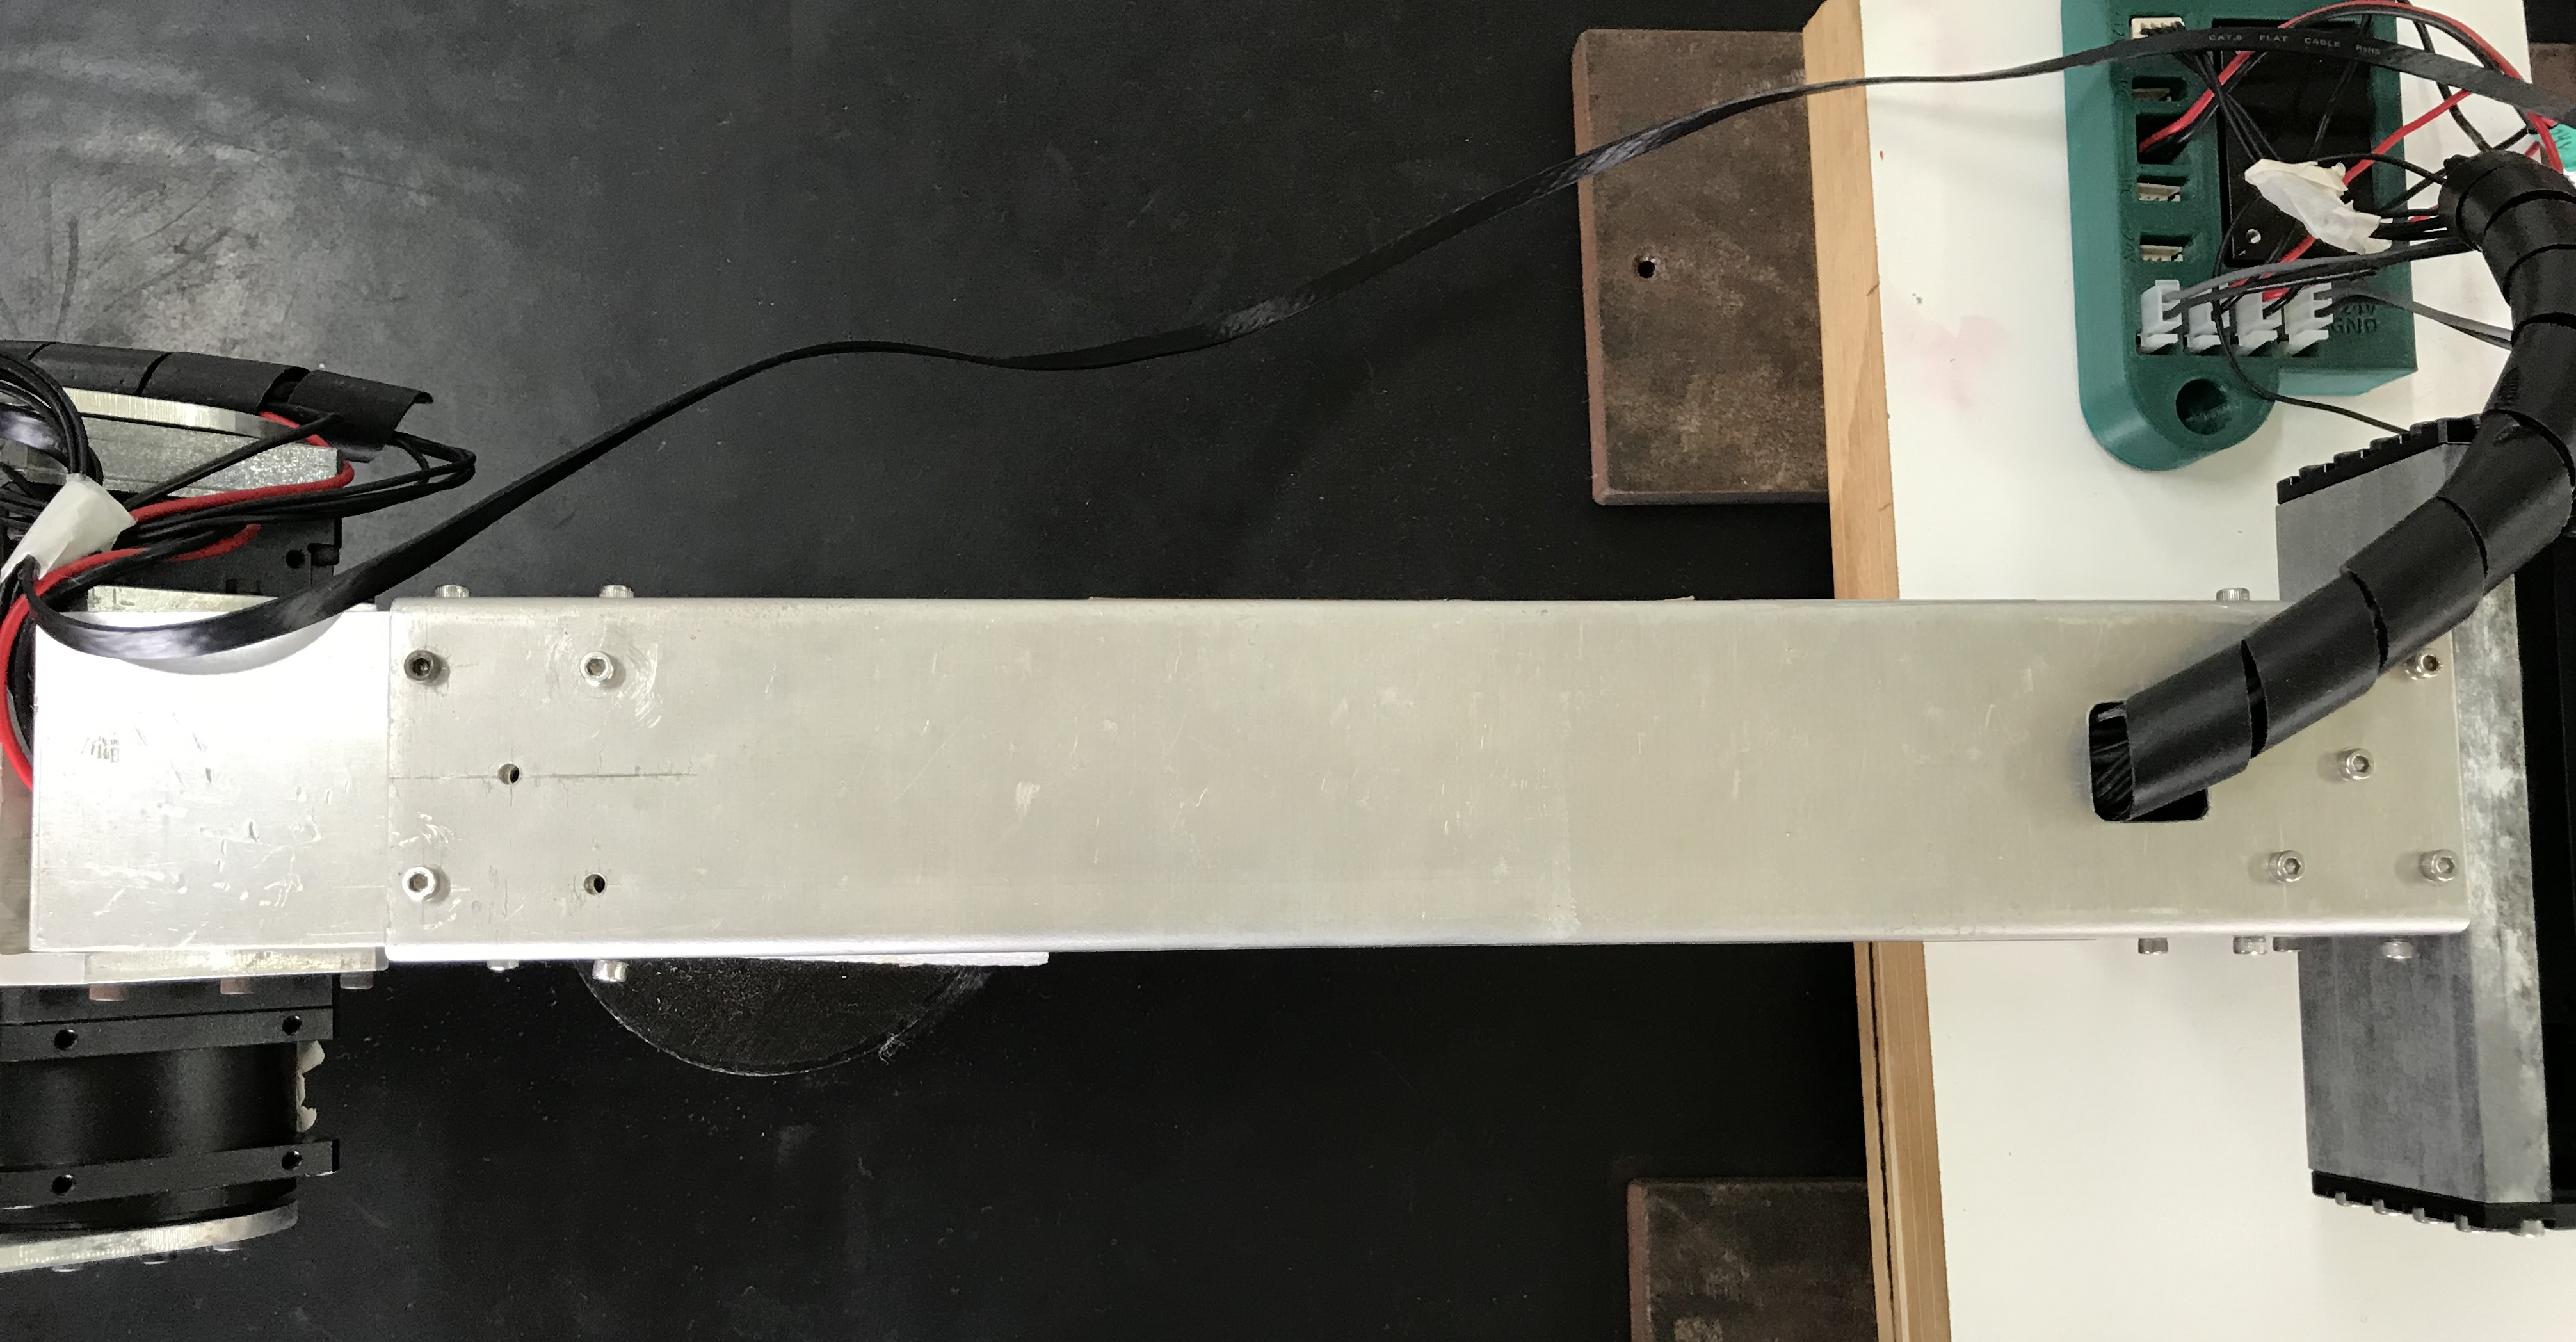
\includegraphics[scale=0.1]{images/elo2.png}
    \legend{Fonte: Autoria própria}
    \label{fig:elo2}
\end{figure}


%------------------------------------------------------------------

\subsection{Suportes}
Foram utilizados suportes com finalidade de unir os elos do manipulador e distribuir movimentos rotativos para as juntas seguintes, feitos em alumínio. Alguns suportes foram adquiridos através da ROBOTIS, enquanto outros foram confeccionados pelo laboratório CCRoSA. A Tabela com os suportes utilizados e suas imagens e medidas pode ser vista no apêndice \ref{apend:frames}.



%------------------------------------------------------------------
\subsection{Câmera}

Para prover o sistema com capacidade de detecção da \emph{tag} e assim obter dados necessários para aquisição de pose e orientação relativa, utilizou-se uma câmera de vídeo modelo Teledyne Genie Nano C2590 (Figura \ref{fig:genie-nano}) e foi acoplada a lente 16mm C Series VIS-NIR (Figura \ref{fig:lens}). A comunicação entre a câmera e o sistema é feita através de um cabo categoria 6 RJ45, e sua ligação pode ser vista no apêndice \ref{apend:connec_schem}.

\begin{figure}[H]
  \centering
  \caption{Teledyne Genie Nano C2590.}
  \includegraphics[scale=0.3]{images/genie-nano.jpg}
  \legend{Fonte: \cite{teledyne}}
  \label{fig:genie-nano}
\end{figure}

\begin{figure}[H]
    \centering
    \caption{Lente 16mm C Series VIS-NIR.}
    \includegraphics[scale=0.8]{images/lens.png}
    \legend{Fonte: \cite{lens}}
    \label{fig:lens}
\end{figure}

Este conjunto pode ser fixado próxima a extremidade do manipulador robótico utilizando um suporte impresso em ABS (Figura \ref{fig:sup-cam}), facilitando a detecção da \emph{tag} e não comprometendo a estrutura do manipulador. O suporte é conectado ao final do \textit{link} 3, como mostra o apêndice \ref{apend:quest}. A integração pode ser visualizada na Figura \ref{fig:int-sup-cam}.

\begin{figure}[H]
    \centering
    \caption{Suporte para fixação da câmera.}
    \includegraphics[scale=0.3]{images/sup-cam.png}
    \legend{Fonte: Autoria própria}
    \label{fig:sup-cam}
\end{figure}

\begin{figure}[H]
    \centering
    \caption{Integração suporte-câmera-lente.}
    \includegraphics[scale=2.5]{images/cam-sup-int.png}
    \legend{Fonte: Autoria própria}
    \label{fig:int-sup-cam}
\end{figure}



%------------------------------------------------------------------
\subsection{Atuadores}

Os atuadores do manipulador são motores de corrente contínua, integrados com redutor de velocidade, controlador e driver. Foram utilizados atuadores \emph{Dynamixel} da fabricante ROBOTIS. Entre os modelos figuram o PH54-200-S500-R, presente nas juntas 0, 1 e 2, o motor PH54-100-S500-R para a junta 3 e o motor PH42-020-S300-R foi utilizado para a junta 4. As especificações do fabricante mais relevantes no projeto estão apresentadas nas tabelas \ref{tab:specs} e \ref{tab:joints_torque}. As folhas de dados estão disponíveis nos anexos \ref{ann:esp_motors_hp42}, \ref{ann:esp_motors_ph54_100} e \ref{ann:esp_motors_ph54_200} para os atuadores PH42-020-S300-R, PH54-100-S500-R, PH54-200-S500-R, respectivamente.

\begin{table}[H]
    \centering
    \caption{Parâmetros dos motores.}
    \resizebox{\columnwidth}{!}{%
    \begin{tabular}{|c|c|c|c|c|c|}
    \hline
    \rowcolor[HTML]{EFEFEF} 
    Tipo & Torque (N.m) & Tensão (V) & Corrente (A) & Velocidade de Rotação (rpm) & Dimensões (mm) \\ \hline
    \rowcolor[HTML]{FFFFFF} 
    PH54-200-S500-R & 44.7 & 24.0 & 9.3 & 29.0 & 54.0 X 126.0 X 54.0 \\ \hline
    \rowcolor[HTML]{EFEFEF} 
    PH54-100-S500-R & 25.3 & 24.0 & 5.5 & 29.2 & 54.0 X 108.0 X 54.0 \\ \hline
    \rowcolor[HTML]{FFFFFF} 
    PH42-020-S300-R & 5.1 & 24.0 & 1.5 & 29.2 & 42.0 X 84.0 X 42.0 \\ \hline
    \end{tabular}
    }

    \label{tab:specs}
    \caption*{Fonte: \cite{dynamixel}}
\end{table}

%------------------------------------------------------------------
\section{Sistema de Potência}
O sistema necessitará ser energizado em dois níveis de tensão, 12 V e 24 V. Durante a realização dos testes, utilizou-se uma fonte com níveis de tensão de 0-30 V e fornecimento de corrente de 0-10 A, para atender os requisitos necessários de potência dos motores. Foi utilizado um conversor DC-DC modelo UWE-12/10-Q12PB-C (Figura \ref{fig:dcdcimg}) na saída da fonte para atingir o nível de tensão de 12 V e energizar a câmera. Um esquema elétrico é fornecido no apêndice \ref{apend:diag_ele}, indicando as conexões dos cabos entre os motores e a câmera.

\begin{figure}[H]
    \centering
    \caption{UWE-12/10-Q12PB-C.}
    \includegraphics[scale=0.20]{images/dcdc.png}
    \legend{Fonte: \cite{dcdc}}
    \label{fig:dcdcimg}
\end{figure}

\section{Comunicação}

O manipulador é conectado via USB através de um disposivo denominado U2D2 \cite{u2d2}. Ele consegue parametrizar e enviar comandos para os motores através dos \textit{softwares} originais da ROBOTIS chamados Dynamixel Workbench e Dynamixel Wizard. O padrão elétrico utilizado é RS-485, ou seja, utiliza-se de 4 fios de conexão que transmitem níveis de tensão e dados. A conexão de entre o computador e os motores, utilizando o U2D2 de intermédio, pode ser vista no apêndice \ref{apend:connec_schem}. A velocidade de transmissão (\textit{baud rate}) definida para todos os motores no sistema é de 57600 bps.

\begin{figure}[H]
    \centering
    \caption{U2D2.}
    \includegraphics[scale=0.70]{images/u2d2.png}
    \legend{Fonte: \cite{u2d2}}
    \label{fig:u2d2img}
\end{figure}


\section{Análise de esforços}
A análise de esforços mecânicos aos quais o manipulador está exposto foi realizada para embasamento e confirmação da capacidade da estrutura e dos atuadores suportarem os esforços de momento torsor. Para isso foram analisadas individualmente as juntas em seus estados críticos. Na Tabela \ref{tab:joints_torque} é apresentada a análise de esforços nas juntas e comparados com os máximos esforços suportados pelos atuadores (conforme vistos nos apêndices \ref{ann:esp_motors_hp42}, \ref{ann:esp_motors_ph54_100} e \ref{ann:esp_motors_ph54_200}), para evitar falhas mecânicas.

Levando em consideração os valores obtidos nas análises de esforços, tem-se as juntas 0 e 1 como juntas críticas do sistema, pois elas sofrem a maior força do sistema e tem o maior torque exigido. Na configuração apresentada, as juntas 0 e 1 suportam a carga máxima de 45.22 N sem chegar a falha mecânica, logo o manipulador possui um limite (\emph{payload}) de aproximadamente 2.1 kg na sua extremidade.

\begin{table}[H]
    \centering
    \caption{Torque das juntas.}
    \resizebox{\columnwidth}{!}{%
    \begin{tabular}{|c|c|c|c|}
    \hline
    \rowcolor[HTML]{EFEFEF} 
    \textbf{Junta} & \textbf{\begin{tabular}[c]{@{}c@{}}Torque máximo fornecido \\ pelos motores (Nm)\end{tabular}} & \textbf{Força resultante na junta (N)} & \textbf{Torque exigido pela junta (Nm)} \\ \hline
    0              & 44.7                                                                                           & 45.22                                  & 25.8                                    \\ \hline
    \rowcolor[HTML]{EFEFEF} 
    1              & 44.7                                                                                           & 45.22                                  & 25.8                                    \\ \hline
    2              & 44.7                                                                                           & 21.44                                  & 6.9                                     \\ \hline
    \rowcolor[HTML]{EFEFEF} 
    3              & 25.3                                                                                           & 4.8                                    & 0.12                                    \\ \hline
    4              & 5.1                                                                                            & 0.87                                   & 0.05                                    \\ \hline
    \end{tabular}
    }
    \label{tab:joints_torque}
    \caption*{Fonte: Autoria própria.}
\end{table}
%------------------------------------------------------------------
%------------------------------------------------------------------
\section{Configurações}
\label{sec:configuracoes}

O conjunto formado pelo manipulador, seu espaço de trabalho e os objetos com os quais ele deverá interagir compõem o sistema abordado neste trabalho. O espaço de trabalho foi representado como uma bancada de 1.70 m $\times$ 0.80 m $\times$ 0.028 m. Há apenas um objeto com o qual o manipulador deverá interagir, uma caixa de dimensões 0.30 m $\times $0.20 m $\times$ 0.20 m.

Para o desafio foi utilizado um marcador visual \textit{ArUco} com dimensões 58x58 mm de id 4, conforme mostrado na Figura \ref{fig:box-real}. Este tem 8 cm do centro do \textit{ArUco} para o botão e 7 cm do centro do \textit{ArUco} para a lâmpada, esta identifica se o botão foi acionado ou não pelo manipulador. 

\begin{figure}[H]
    \centering
    \caption{Caixa objetivo.}
    \includegraphics[scale=1.8]{images/box-real.png}
    \legend{Fonte: Autoria própria}
    \label{fig:box-real}
\end{figure}



O manipulador possui a posição home definida como da Figura \ref{fig:home_position} onde o ângulo de cada motor está descrito na Tabela \ref{tab:home_position}.

\begin{figure}[H]
    \centering
    \caption{Manipulador na posição home.}
    \includegraphics[scale=0.4]{images/home_position.jpg}
    \label{fig:home_position}
    \caption*{Fonte: Autoria própria.}
\end{figure}

\begin{table}[H]
    \centering
    \caption{Ângulos dos motores na posição home.}
    \begin{tabular}{|c|c|}
    \hline
    \rowcolor[HTML]{EFEFEF} 
    \textbf{Motor} & \textbf{Ângulo}                           \\ \hline
    \rowcolor[HTML]{FFFFFF} 
    ID\_1          & $0^\circ$   \\ \hline
    ID\_2          & $-24^\circ$ \\ \hline
    \rowcolor[HTML]{FFFFFF} 
    ID\_3          & $141^\circ$ \\ \hline
    ID\_4          & $0^\circ$   \\ \hline
    \rowcolor[HTML]{FFFFFF} 
    ID\_5          & $0^\circ$   \\ \hline
    \end{tabular}
    \label{tab:home_position}
    \caption*{Fonte: Autoria própria.}
    \end{table}


